\documentclass[crop,border={2pt 2pt 2pt 2pt},tikz]{standalone}
\usepackage{braket}
\usepackage{bbold}
\usepackage{bm}
\usepackage{amsmath}
\usepackage{tikz-3dplot}
% \usepackage{physics}

\usetikzlibrary{backgrounds,decorations.markings, calc}
\tikzset{>=latex}
\tikzset{->-/.style={decoration={
  markings,
  mark=at position .55 with {\arrow{>}}},postaction={decorate}}}
\begin{document}
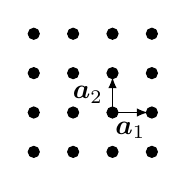
\begin{tikzpicture}[line join = round]
    \foreach \i in {0,0.5,...,1.5}{
        \foreach \j in {0,0.5,...,1.5}{
            \draw[fill,black] (\i,\j) circle (2pt);
        }
    }
    \draw[->] (1,0.5) -- node[anchor=north, pos=0.5] {$\bm a_1$} (1.45,0.5);
    \draw[->] (1,0.5) -- node[anchor=east, pos=0.5] {$\bm a_2$} (1,0.95);
\end{tikzpicture}
\end{document}